\chapter{System Design}

This chapter presents the design of UltraFabric-Vision. It states the functional and performance specifications, describes the parallel three-pathway architecture, derives the calibration and fusion equations that turn three heterogeneous detectors into a single decision, and outlines the deployment design that exposes the system to factory software.

\section{Design Specifications}

The system is designed to meet the following specifications:
\begin{enumerate}
\item Operate on a fixed input of $224\times224$ RGB frames.
\item Require only defect-free fabric for fitting and calibration (no labelled defects).
\item Produce a single scalar anomaly score and a spatial defect heatmap per frame.
\item Achieve real-time throughput ($\geq 15$~FPS) on a consumer GPU.
\item Expose a network interface for line integration and an embeddable interface for edge integration.
\end{enumerate}

\section{Architecture Overview}

The architecture comprises three detection pathways operating in parallel on the same preprocessed input, followed by a calibration-and-fusion stage. Each pathway independently produces a scalar score and a heatmap; the scores are standardized and averaged into a single decision variable, and the heatmaps are normalized and averaged into a fused localization map. Figure~\ref{fig:arch} depicts the end-to-end flow.

\begin{figure}[htb]
\centering
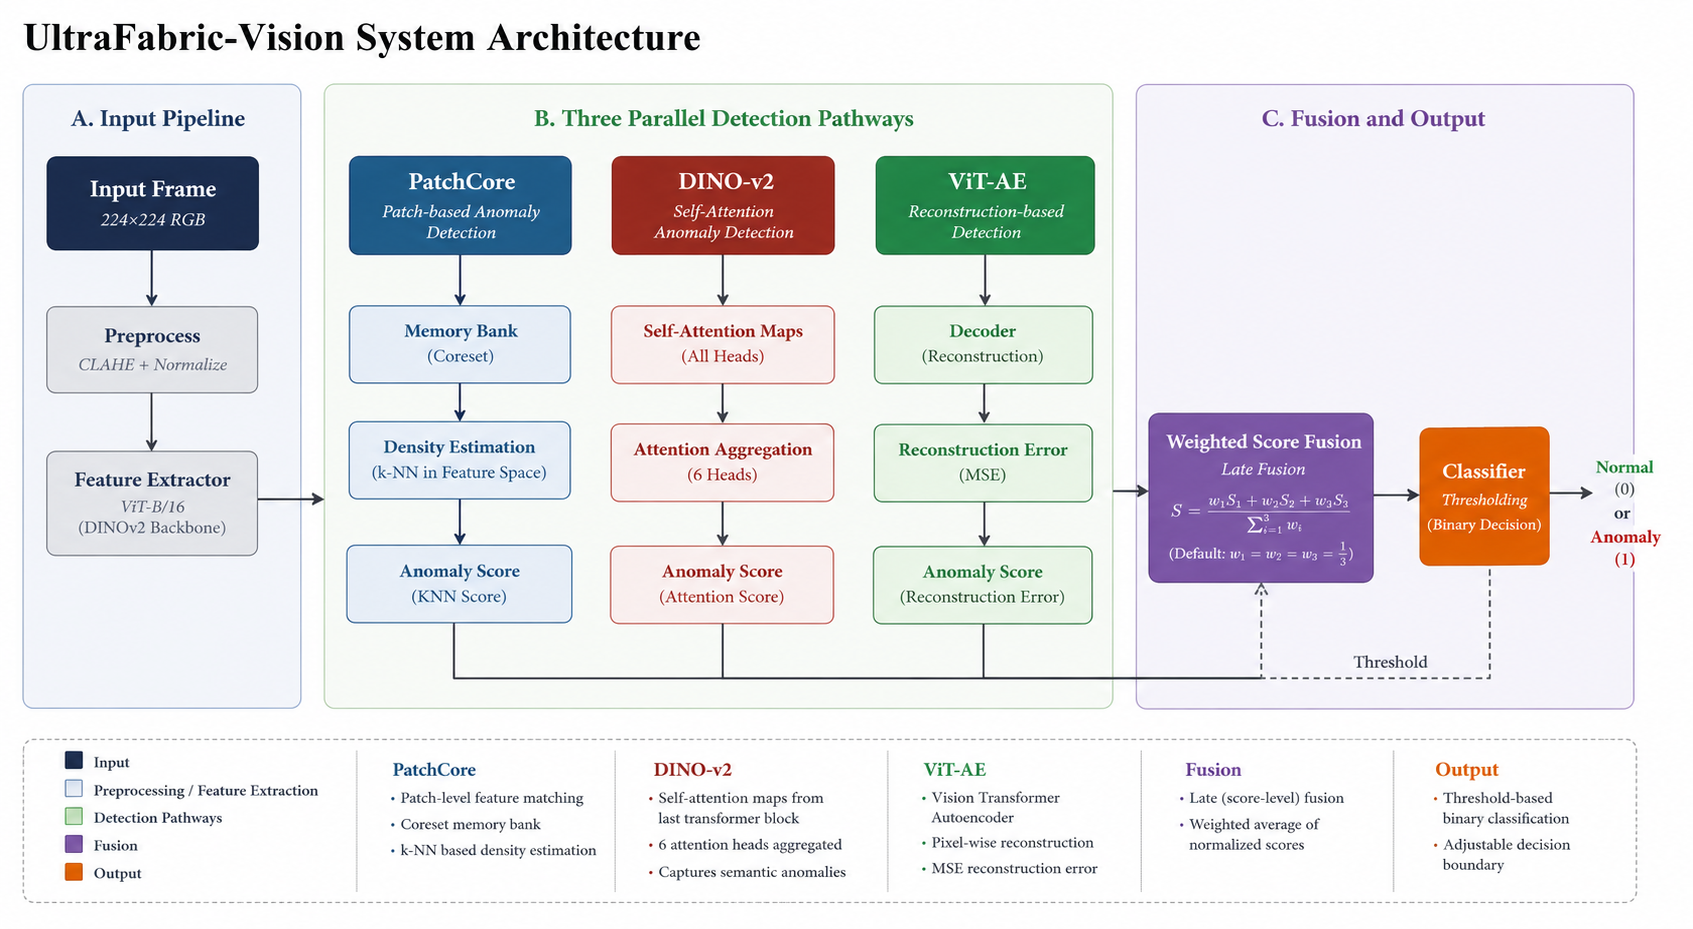
\includegraphics[width=0.95\textwidth]{Figures/system_architecture.png}
\caption{End-to-end architecture: shared preprocessing feeds three parallel detectors (PatchCore, DINO, ViT-Autoencoder) whose calibrated scores and heatmaps are fused into a single decision and localization map.}
\label{fig:arch}
\end{figure}

\section{Preprocessing Design}

A single preprocessing routine is shared, byte-for-byte, between fitting and inference: resize to $224\times224$, convert to a tensor, and normalize using ImageNet statistics
\[
\hat{\mathbf{x}} = \frac{\mathbf{x}/255 - \boldsymbol{\mu}}{\boldsymbol{\sigma}}, \quad
\boldsymbol{\mu} = [0.485,0.456,0.406],\ \boldsymbol{\sigma} = [0.229,0.224,0.225].
\]
Enhancement operators (contrast equalization, blur, letterbox padding) are deliberately excluded because they are not applied at fit time; introducing them only at inference shifts every frame off the fitted manifold and collapses accuracy.

\section{Calibration and Fusion Design}

Let $\hat{s}_m(\mathbf{x})$ be the raw score of detector $m\in\{\text{PC},\text{D},\text{VAE}\}$. Over a calibration set of defect-free images $\mathcal{D}_{\text{cal}}$ we estimate the per-detector statistics
\[
\mu_m = \frac{1}{|\mathcal{D}_{\text{cal}}|}\sum_{\mathbf{x}} \hat{s}_m(\mathbf{x}), \qquad
\sigma_m = \sqrt{\frac{1}{|\mathcal{D}_{\text{cal}}|}\sum_{\mathbf{x}} (\hat{s}_m(\mathbf{x})-\mu_m)^2},
\]
and standardize each score to a z-score,
\[
z_m(\mathbf{x}) = \frac{\hat{s}_m(\mathbf{x}) - \mu_m}{\sigma_m}.
\]
The ensemble decision score and fused heatmap are the (uniformly) weighted averages
\[
\hat{s}_{\text{ens}} = \sum_m w_m\, z_m, \qquad
\mathbf{H}_{\text{ens}} = \sum_m w_m\, \mathbf{H}^{\text{norm}}_m, \qquad \sum_m w_m = 1.
\]
A frame is declared defective when $\hat{s}_{\text{ens}} > \tau$, with the threshold $\tau$ fixed by maximizing Youden's J statistic, $\tau^\star = \arg\max_\tau [\text{TPR}(\tau) - \text{FPR}(\tau)]$, on a validation set. Because each $z_m$ is centered on defect-free cloth, $\hat{s}_{\text{ens}}$ is near zero for normal fabric and $\tau$ is expressed in interpretable standard-deviation units.

\section{Deployment Design}

The calibrated pipeline is packaged behind three interfaces sharing one engine: a FastAPI REST/WebSocket server for line integration and live dashboards, an embeddable Python SDK for edge/PLC integration, and a batch command-line tool that emits CSV/JSON reports for manufacturing-execution systems. Runtime behaviour (device, mixed precision, threshold source, network binding, authentication) is controlled entirely through environment variables so that a single container image runs unchanged from development to the factory floor.

In summary, the design combines a diverse three-pathway detector bank with a principled calibration-and-fusion stage and a deployment-oriented interface layer. Chapter~4 describes how each of these design elements is realized in code.
